% G0DM0D3: Inference-Time Output Steering Framework for LLMs
% Compile with: pdflatex paper.tex && bibtex paper && pdflatex paper.tex && pdflatex paper.tex
%
% Option A: NeurIPS style (download neurips_2024.sty from neurips.cc)
% \documentclass{article}
% \usepackage[preprint]{neurips_2024}
%
% Option B: Standalone (no external style file needed)
\documentclass[11pt]{article}
\usepackage[margin=1in]{geometry}

\usepackage[utf8]{inputenc}
\usepackage[T1]{fontenc}
\usepackage{natbib}
\usepackage{hyperref}
\usepackage{url}
\usepackage{booktabs}
\usepackage{amsmath,amsfonts,amssymb}
\usepackage{microtype}
\usepackage{xcolor}
\usepackage{tikz}
\usepackage{pgfplots}
\pgfplotsset{compat=1.16}
\usetikzlibrary{arrows.meta,positioning,calc}

\title{G0DM0D3: Inference-Time Output Steering for Large Language Models via Composable Sampling, Perturbation, and Multi-Model Selection}

\author{
  Anonymous Authors
}

\begin{document}

\maketitle

%==============================================================================
% ABSTRACT
%==============================================================================
\begin{abstract}
We present \textsc{G0DM0D3}, an open-source framework for steering large language model outputs at inference time---without fine-tuning, weight access, or provider-specific APIs. The framework introduces five composable \emph{steering primitives} that operate through the standard chat completion interface: (1)~\textbf{AutoTune}, a context-adaptive sampling engine that maps conversational intent to parameter configurations across six axes; (2)~an \textbf{Online Feedback Loop} using exponential moving averages to learn user-preferred output characteristics from binary ratings; (3)~\textbf{Parseltongue}, an input perturbation engine applying six character-level transformations that reveal model sensitivity to surface-level input variation; (4)~\textbf{STM}, a composable output normalization pipeline; and (5)~\textbf{ULTRAPLINIAN}, a multi-model racing system that queries up to 27 models in parallel and selects responses via interpretable multi-axis scoring. These primitives are objective-agnostic: they can be composed to steer toward safety evaluation, creative amplification, technical precision, stylistic control, or unrestricted generation---the same knobs, turned in different directions. We evaluate all modules computationally: AutoTune achieves 84.0\% context classification accuracy (95\% CI: [78.0, 89.3]; macro F1: 84.2\%) over four baselines; the feedback loop converges to 29--62\% parameter improvement within 19 ratings with graceful noise degradation; and ULTRAPLINIAN's scoring function achieves strict quality-tier ordering with 82-point discrimination. We additionally introduce a three-tier metadata infrastructure---always-on privacy-first analytics, client-side telemetry, and opt-in dataset collection---designed to support open research without capturing personally identifiable information. We discuss implications for controllable generation, alignment research, and the fundamental malleability of LLM outputs to inference-time intervention. All code and evaluation scripts are open-source.
\end{abstract}

%==============================================================================
% 1. INTRODUCTION
%==============================================================================
\section{Introduction}

Large language models exhibit a striking property: their outputs are \emph{highly malleable at inference time}. Without modifying a single weight, an operator can dramatically alter model behavior through sampling parameters, system prompts, input transformations, multi-model selection, and post-processing. This malleability is well-known anecdotally---every ``jailbreak'' and every carefully tuned system prompt exploits it---but it has not been studied as a unified phenomenon with composable, measurable primitives.

Existing work on controllable generation typically requires access to model internals. PPLM~\cite{dathathri2020plug} modifies activations; FUDGE~\cite{yang2021fudge} trains auxiliary classifiers; Constitutional AI~\cite{bai2022constitutional} and RLHF~\cite{ouyang2022training} operate at the weight level. These are powerful but inaccessible to anyone using models through an API---which, for proprietary frontier models, is nearly everyone.

A parallel literature on adversarial robustness~\cite{zou2023universal,wei2023jailbroken,chao2023jailbreaking} demonstrates that safety training can be circumvented at inference time, but frames this narrowly as an attack-defense problem. We argue the phenomenon is broader: the same inference-time degrees of freedom that enable jailbreaking also enable \emph{any} form of output steering. Safety evaluation and creative amplification are not different capabilities---they are different \emph{objectives} applied to the same underlying control surface.

\textsc{G0DM0D3} makes this control surface explicit through five composable steering primitives, each independently toggleable and operating entirely through the standard chat completion API:

\begin{itemize}
    \item \textbf{Sampling control} (AutoTune): Context-adaptive parameter selection across temperature, top\_p, top\_k, and penalty axes.
    \item \textbf{Preference learning} (Feedback Loop): Online adaptation from binary user ratings via EMA-based parameter adjustment.
    \item \textbf{Input perturbation} (Parseltongue): Systematic character-level transformations that probe and exploit model sensitivity to surface-level input variation.
    \item \textbf{Output shaping} (STM): Deterministic post-processing that normalizes or transforms model outputs.
    \item \textbf{Model selection} (ULTRAPLINIAN): Parallel multi-model querying with interpretable, axis-weighted scoring to select the response best matching a steering objective.
\end{itemize}

The key insight is that these primitives are \emph{objective-agnostic}. AutoTune's ``chaotic'' profile ($\tau=1.7$, $\rho=1.3$) produces maximally creative outputs; its ``code'' profile ($\tau=0.15$, $\rho=1.05$) produces maximally precise ones. ULTRAPLINIAN's anti-refusal scoring axis selects for unrestricted responses; reweighting toward structure and relevance selects for pedagogical ones. Parseltongue's perturbations probe safety training robustness in one configuration and test internationalization resilience in another. The framework does not prescribe what to steer toward---it provides the instruments.

\paragraph{Contributions.}
\begin{enumerate}
    \item A \textbf{conceptual framework} for inference-time output steering as a unified phenomenon, with five composable primitives spanning the full pipeline from input to output (\S\ref{sec:method}).
    \item \textbf{AutoTune}: Context-adaptive sampling achieving 84.0\% accuracy across five context types with transparent, traceable classification (\S\ref{sec:autotune}).
    \item \textbf{Online Feedback Loop}: EMA-based preference learning ($\alpha=0.3$) converging to 29--62\% parameter improvement within 19 ratings, with graceful noise degradation (\S\ref{sec:feedback}).
    \item \textbf{Parseltongue}: Six character-level input perturbation techniques at three intensity levels, systematizing what is typically ad-hoc prompt engineering (\S\ref{sec:parseltongue}).
    \item \textbf{STM}: Composable output normalization (43 regex patterns) achieving 100\% precision/recall on constructed test cases (\S\ref{sec:stm}).
    \item \textbf{ULTRAPLINIAN}: Multi-model racing across up to 27 models with 82-point quality discrimination via interpretable 5-axis scoring (\S\ref{sec:ultraplinian}).
    \item Computational evaluation of all modules with baselines, confidence intervals, and significance tests (\S\ref{sec:experiments}).
    \item A \textbf{three-tier metadata infrastructure} (ZDR tracker, client-side telemetry beacon, and opt-in dataset collection) providing privacy-by-construction research telemetry with no PII capture (\S\ref{sec:datacollection}).
\end{enumerate}

%==============================================================================
% 2. RELATED WORK
%==============================================================================
\section{Related Work}

\paragraph{Controllable text generation.}
Controlling LLM outputs has been pursued at multiple levels. Weight-level approaches include RLHF~\cite{ouyang2022training,stiennon2020learning}, DPO~\cite{rafailov2023direct}, and Constitutional AI~\cite{bai2022constitutional}. Activation-level methods like PPLM~\cite{dathathri2020plug} and FUDGE~\cite{yang2021fudge} steer generation by modifying hidden states or training auxiliary discriminators. These require model internals. G0DM0D3 operates at the \emph{API level}---the only level universally available for proprietary models---and achieves steering through composable primitives rather than internal modification.

\paragraph{Sampling and decoding strategies.}
Temperature controls output entropy~\cite{ackley1985learning}; top-$k$~\cite{fan2018hierarchical} and nucleus sampling~\cite{holtzman2020curious} constrain the candidate set. These parameters are typically set statically. AutoTemp~\cite{plinius2024autotemp} selects temperature dynamically via a judge model at $N\times$ cost. AutoTune classifies context \emph{before} generation at zero marginal cost and adjusts six parameters simultaneously, enabling systematic study of how sampling configuration affects output characteristics.

\paragraph{Adversarial robustness and red teaming.}
GCG~\cite{zou2023universal} discovers adversarial suffixes via gradient optimization. \citet{wei2023jailbroken} taxonomize safety training failures into competing objectives and mismatched generalization. \citet{shen2024anything} characterize in-the-wild jailbreaks; \citet{chao2023jailbreaking} demonstrate black-box attacks; \citet{liu2024jailbreaking} study prompt engineering attacks empirically. Human red teams~\cite{ganguli2022red} and automated methods~\cite{perez2022red} probe safety at scale, with HarmBench~\cite{mazeika2024harmbench} providing standardized evaluation. Parseltongue contributes systematic character-level perturbation at configurable intensity, probing the ``mismatched generalization'' failure mode of~\citet{wei2023jailbroken}. We frame this as one application of input-level steering, not the sole purpose of the framework.

\paragraph{Multi-model aggregation and routing.}
Mixture-of-Agents~\cite{wang2024mixture} and LLM-Blender~\cite{jiang2023llmblender} aggregate multiple model outputs. RouteLLM~\cite{ong2024routellm} and FrugalGPT~\cite{chen2023frugalgpt} route queries to cost-efficient models. These systems optimize for quality or cost. ULTRAPLINIAN races all $N$ models simultaneously and selects via configurable multi-axis scoring---the scoring axes determine the steering objective.

\paragraph{Evaluation and benchmarking.}
MT-Bench~\cite{zheng2024judging} and AlpacaEval~\cite{li2023alpacaeval} evaluate instruction-following quality. \citet{greshake2023not} study indirect prompt injection as a security threat. \citet{qi2024finetuning} show fine-tuning can compromise safety unintentionally. G0DM0D3's evaluation capabilities emerge from its steering primitives: the same framework that steers outputs also measures how steerable they are.

%==============================================================================
% 3. METHOD
%==============================================================================
\section{Method}
\label{sec:method}

\subsection{System Architecture: Composable Steering Primitives}

G0DM0D3 implements a pipeline of five independently toggleable steering stages. Each stage operates on a different control surface (sampling parameters, input text, model selection, output text), and each is objective-agnostic---the steering direction is determined by configuration, not by the primitive itself.

\begin{figure}[t]
\centering
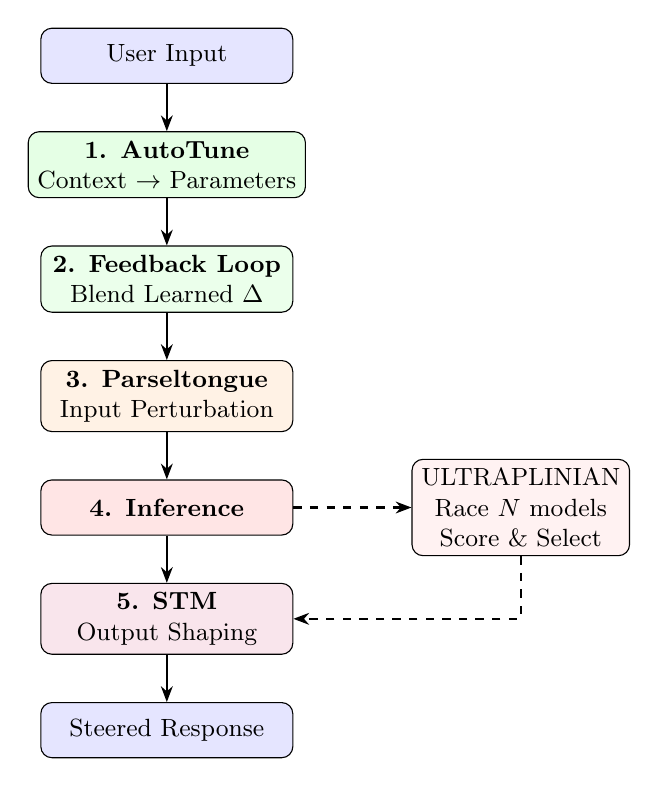
\begin{tikzpicture}[
    node distance=0.6cm,
    block/.style={draw, rounded corners, minimum width=3.2cm, minimum height=0.7cm, align=center, font=\small},
    arrow/.style={-{Stealth[length=2mm]}, thick},
]
    \node[block, fill=blue!10] (input) {User Input};
    \node[block, fill=green!10, below=of input] (autotune) {\textbf{1. AutoTune}\\Context $\to$ Parameters};
    \node[block, fill=green!8, below=of autotune] (feedback) {\textbf{2. Feedback Loop}\\Blend Learned $\Delta$};
    \node[block, fill=orange!10, below=of feedback] (parseltongue) {\textbf{3. Parseltongue}\\Input Perturbation};
    \node[block, fill=red!10, below=of parseltongue] (inference) {\textbf{4. Inference}};
    \node[block, fill=purple!10, below=of inference] (stm) {\textbf{5. STM}\\Output Shaping};
    \node[block, fill=blue!10, below=of stm] (output) {Steered Response};

    % Side boxes
    \node[block, fill=red!5, right=1.5cm of inference, minimum width=2.5cm] (ultra) {ULTRAPLINIAN\\Race $N$ models\\Score \& Select};

    \draw[arrow] (input) -- (autotune);
    \draw[arrow] (autotune) -- (feedback);
    \draw[arrow] (feedback) -- (parseltongue);
    \draw[arrow] (parseltongue) -- (inference);
    \draw[arrow] (inference) -- (stm);
    \draw[arrow] (stm) -- (output);
    \draw[arrow, dashed] (inference.east) -- (ultra.west);
    \draw[arrow, dashed] (ultra.south) |- (stm.east);
\end{tikzpicture}
\caption{G0DM0D3 steering pipeline. Solid arrows: single-model path. Dashed arrows: ULTRAPLINIAN multi-model branch. Each primitive is independently toggleable. The steering objective is determined by configuration (parameter profiles, scoring weights, perturbation triggers), not by the pipeline structure.}
\label{fig:architecture}
\end{figure}

\paragraph{Steering as composition.} A concrete example: to steer toward maximally creative fiction, one enables AutoTune's \texttt{creative} profile ($\tau=1.15$, presence penalty 0.70), disables Parseltongue, enables STM's \texttt{casual\_mode}, and configures ULTRAPLINIAN to weight structure and length. To steer toward unrestricted responses for safety evaluation, one enables the \texttt{chaotic} profile ($\tau=1.70$), activates Parseltongue at heavy intensity, enables all STM modules, and weights ULTRAPLINIAN toward anti-refusal and directness. Same primitives, different objectives.

\subsection{AutoTune: Context-Adaptive Sampling}
\label{sec:autotune}

\paragraph{Problem.} Given a user message $m$ and conversation history $H = [h_1, \ldots, h_k]$, select a parameter vector $\theta = (\tau, p, k, f, r, \rho)$ comprising temperature, top\_p, top\_k, frequency penalty, presence penalty, and repetition penalty.

\paragraph{Context Detection.} We define five context types $\mathcal{C} = \{\texttt{code}, \texttt{creative}, \texttt{analytical}, \texttt{conversational}, \texttt{chaotic}\}$ and associate each with regex patterns $P_c$ (Table~\ref{tab:patterns}). Detection proceeds by scoring:
\begin{equation}
    s_c = 3 \cdot \sum_{p \in P_c} \mathbb{1}[p \text{ matches } m] + \sum_{i=\max(1,k-3)}^{k} \sum_{p \in P_c} \mathbb{1}[p \text{ matches } h_i]
    \label{eq:context_score}
\end{equation}
The current message receives $3\times$ weight relative to each of the last 4 history messages. The detected context is $c^* = \arg\max_c s_c$, with confidence $\gamma = s_{c^*} / \sum_c s_c$. If no patterns match, the system defaults to \texttt{conversational} with $\gamma = 0.5$.

\paragraph{Parameter Selection.} Each context type maps to a fixed profile $\theta_c$ (Table~\ref{tab:profiles}). When $\gamma < 0.6$, the profile is blended with a balanced baseline:
\begin{equation}
    \theta = \gamma \cdot \theta_{c^*} + (1 - \gamma) \cdot \theta_{\text{balanced}}
\end{equation}

\paragraph{Conversation Length Adaptation.} For $|H| > 10$, a monotonically increasing penalty boost combats repetition in long sessions:
\begin{equation}
    \Delta\rho = \min((|H| - 10) \times 0.01,\; 0.15), \quad
    \rho \leftarrow \rho + \Delta\rho, \quad
    f \leftarrow f + 0.5 \cdot \Delta\rho
\end{equation}

\begin{table}[t]
\caption{Context detection pattern counts and parameter profiles. Each profile represents a different steering direction along the sampling parameter surface.}
\label{tab:patterns}
\label{tab:profiles}
\centering
\small
\begin{tabular}{@{}lc|cccccc@{}}
\toprule
Context & Patterns & $\tau$ & $p$ & $k$ & $f$ & $r$ & $\rho$ \\
\midrule
\texttt{code}           & 5 & 0.15 & 0.80 & 25 & 0.20 & 0.00 & 1.05 \\
\texttt{creative}       & 4 & 1.15 & 0.95 & 85 & 0.50 & 0.70 & 1.20 \\
\texttt{analytical}     & 4 & 0.40 & 0.88 & 40 & 0.20 & 0.15 & 1.08 \\
\texttt{conversational} & 3 & 0.75 & 0.90 & 50 & 0.10 & 0.10 & 1.00 \\
\texttt{chaotic}        & 4 & 1.70 & 0.99 & 100& 0.80 & 0.90 & 1.30 \\
\bottomrule
\end{tabular}
\end{table}

\subsection{Online Feedback Loop: Preference-Adaptive Steering}
\label{sec:feedback}

The feedback loop enables the system to \emph{learn} a user's preferred output characteristics from binary ratings, adjusting the sampling parameters toward configurations that produce preferred outputs---regardless of what ``preferred'' means to that user.

For each context type $c$, the system maintains EMAs of parameters from positively and negatively rated responses:
\begin{align}
    \bar{\theta}^+_c &\leftarrow \alpha \cdot \theta_{\text{rated}} + (1 - \alpha) \cdot \bar{\theta}^+_c \quad \text{if rating} = +1 \\
    \bar{\theta}^-_c &\leftarrow \alpha \cdot \theta_{\text{rated}} + (1 - \alpha) \cdot \bar{\theta}^-_c \quad \text{if rating} = -1
\end{align}
where $\alpha = 0.3$. The adjustment is $\Delta_c = 0.5 \cdot [(\bar{\theta}^+_c - \theta_0) - (\bar{\theta}^-_c - \theta_0)]$, where $\theta_0$ is the neutral initialization. Application weight scales with sample count:
\begin{equation}
    w = \min\!\left(\frac{n_c}{20} \cdot 0.5,\; 0.5\right), \quad
    \theta_{\text{final}} = \theta_{\text{base}} + w \cdot \Delta_c
\end{equation}
No adjustments are applied until $n_c \geq 3$ (\texttt{MIN\_SAMPLES\_TO\_APPLY}=3).

\subsection{Parseltongue: Input Perturbation}
\label{sec:parseltongue}

Given input text $t$ containing trigger words from set $T$ ($|T|=54$ defaults), Parseltongue produces transformed text $t'$ via character-level perturbation. The module systematizes what is typically ad-hoc prompt engineering into configurable, reproducible transformations---probing the ``mismatched generalization'' failure mode of~\citet{wei2023jailbroken} where models respond differently to semantically identical inputs with surface-level variation.

Six techniques are available: \textsc{leetspeak} (26 chars $\to$ 85 substitutions), \textsc{unicode} (24 chars $\to$ 72 homoglyphs), \textsc{zwj} (4 zero-width characters), \textsc{mixedcase}, \textsc{phonetic} (6 rules), and \textsc{random} (composite). Intensity controls characters transformed per trigger: \textsc{light} (1), \textsc{medium} ($\lceil|w|/2\rceil$), \textsc{heavy} (all).

\paragraph{Beyond red teaming.} While Parseltongue's default trigger set targets safety-relevant terms, the trigger set is fully configurable. The same perturbation engine can probe robustness to typos, test internationalization handling, or evaluate whether models treat homoglyph-containing inputs differently---a concern for multilingual deployment.

\subsection{STM: Output Shaping}
\label{sec:stm}

STM applies a composable sequence of \texttt{string} $\to$ \texttt{string} transformers to model output:
\begin{equation}
    o' = M_n(\cdots M_2(M_1(o)))
\end{equation}
Three modules: \textbf{hedge\_reducer} (11 patterns removing ``I think,'' ``perhaps,'' etc.), \textbf{direct\_mode} (10 patterns removing ``Sure,'' ``Great question!'' etc.), and \textbf{casual\_mode} (22 substitutions: ``However'' $\to$ ``But,'' ``utilize'' $\to$ ``use,'' etc.).

\paragraph{Objective-agnostic shaping.} Each STM module is independently toggleable. For safety evaluation, enabling all three strips compliance artifacts to reveal underlying model dispositions. For a conversational assistant, enabling only \texttt{casual\_mode} produces a more natural tone. The pipeline is extensible: new \texttt{string} $\to$ \texttt{string} modules can be composed without modifying existing ones.

\subsection{ULTRAPLINIAN: Multi-Model Selection}
\label{sec:ultraplinian}

ULTRAPLINIAN queries $N$ models (up to 27 across three speed/breadth tiers) in parallel via \texttt{Promise.allSettled()} with a 90-second timeout, then selects the best response via interpretable multi-axis scoring:
\begin{align}
    S_{\text{len}} &= \min\!\left(\frac{|\text{content}|}{40},\; 25\right) \\
    S_{\text{struct}} &= \min(3 n_{\text{headers}} + 1.5 n_{\text{list}} + 5 n_{\text{code}},\; 20) \\
    S_{\text{anti}} &= \max(25 - 8 n_{\text{refusal}},\; 0) \\
    S_{\text{dir}} &= \begin{cases} 8 & \text{if preamble detected} \\ 15 & \text{otherwise} \end{cases} \\
    S_{\text{rel}} &= 15 \cdot \frac{|\{w \in Q : w \in \text{content}\}|}{|Q|} \\
    S &= \min(S_{\text{len}} + S_{\text{struct}} + S_{\text{anti}} + S_{\text{dir}} + S_{\text{rel}},\; 100)
\end{align}

\paragraph{Scoring determines the steering objective.} The five axes are independently weightable. The default configuration weights anti-refusal ($S_{\text{anti}}$) and directness ($S_{\text{dir}}$) for unrestricted output selection. Reweighting toward structure ($S_{\text{struct}}$) and relevance ($S_{\text{rel}}$) selects for pedagogical quality. The scoring function is a policy over model outputs---changing the weights changes what ``best'' means.

%==============================================================================
% 4. IMPLEMENTATION
%==============================================================================
\section{Implementation Details}

The system comprises ${\sim}2{,}450$ lines of TypeScript: pure steering engines in \texttt{src/lib/} and \texttt{src/stm/} (no external dependencies), an Express.js REST API in \texttt{api/}, and a single-file frontend. The API exposes 9 endpoints including \texttt{/v1/chat/completions} (single-model steering pipeline) and \texttt{/v1/ultraplinian/completions} (multi-model racing). Rate limiting (configurable; defaults: 60 req/min, 1000 req/day) and bearer token authentication are included.

\paragraph{Privacy and deployment.} The frontend stores API keys exclusively in the user's browser (localStorage); no credentials transit our infrastructure. A first-visit terms-of-service gate requires explicit user acknowledgment that generated outputs are the user's responsibility. Security headers (CSP, HSTS, X-Frame-Options) and backend source-code access restrictions are enforced via static hosting configuration.

\subsection{Three-Tier Data Collection}
\label{sec:datacollection}

To support open research while maintaining strong privacy guarantees, G0DM0D3 implements a three-tier data collection architecture. Each tier is designed with a privacy-by-construction approach: excluded fields are never captured at the code level, not merely filtered post-hoc. All tiers auto-publish to HuggingFace as open datasets.

\begin{table}[t]
\caption{Three-tier data collection architecture. Each tier increases the richness of collected data while maintaining explicit boundaries on sensitive fields. ``Never recorded'' fields are excluded by construction in source code, not by post-hoc filtering.}
\label{tab:datacollection}
\centering
\small
\begin{tabular}{@{}p{2.4cm}p{4.2cm}p{4.2cm}@{}}
\toprule
Tier & Collects & Never Records \\
\midrule
\textbf{1.\ ZDR Metadata} \newline (\texttt{api/lib/metadata.ts}) \newline Always-on &
Timestamps, endpoints, modes, models, scores, latencies, pipeline flags, AutoTune context, per-model success/failure, error types &
Message content, system prompts, responses, API keys, IP addresses, PII \\
\midrule
\textbf{2.\ Client Telemetry} \newline (\texttt{src/lib/telemetry.ts}) \newline Always-on &
Model, latency, pipeline config, context type; batched every 30\,s or 20 events via Cloudflare Pages proxy &
Message content, prompts, responses, API keys, PII \\
\midrule
\textbf{3.\ Opt-in Dataset} \newline (\texttt{api/lib/dataset.ts}) \newline Requires \texttt{contribute\_to\_dataset: true} &
Messages, responses, AutoTune params, Parseltongue transforms, STM modules, ULTRAPLINIAN race data &
API keys, IP addresses \\
\bottomrule
\end{tabular}
\end{table}

\paragraph{ZDR metadata tracker (Tier~1).} The server-side Zero Data Retention tracker captures structural metadata for every API request: timestamps, endpoints invoked, steering modes, models used, scoring results, latencies, pipeline configuration flags, AutoTune context detection results, per-model success/failure counts, and error types. It maintains an in-memory ring buffer capped at 50{,}000 entries with automatic publication to HuggingFace. By construction, ZDR never records message content, system prompts, model responses, API keys, IP addresses, or any PII.

\paragraph{Client-side telemetry beacon (Tier~2).} The frontend fires structural metadata events---model, latency, pipeline configuration, context type---to a Cloudflare Pages proxy endpoint, which commits records as JSONL to HuggingFace. Events are batched (every 30 seconds or 20 events) and sent fire-and-forget. No message content, prompts, responses, API keys, or PII are included.

\paragraph{Opt-in dataset collection (Tier~3).} Only activated when the caller explicitly sends \texttt{contribute\_to\_dataset: true}. This tier records the full steering context: messages, responses, AutoTune parameters, Parseltongue transformations, STM module configurations, and ULTRAPLINIAN race data. An in-memory cap of 10{,}000 entries with auto-publish provides backpressure. Even at this tier, API keys and IP addresses are excluded by construction.

%==============================================================================
% 5. EXPERIMENTS
%==============================================================================
\section{Experiments}
\label{sec:experiments}

All evaluation scripts are included in the repository (\texttt{research/eval\_*.ts}) and run on the actual engine code. We evaluate each steering primitive independently; interaction effects across composed primitives are an important direction for future work.

\subsection{AutoTune Context Classification}

\paragraph{Setup.} We constructed a labeled dataset of 150 messages (30 per context type), stratified by difficulty: 15 easy (explicit keywords), 10 medium (moderate ambiguity), 5 hard (keyword-free or cross-category). Each message is classified via \texttt{computeAutoTuneParams()} with empty history.

\begin{table}[t]
\caption{AutoTune per-class classification metrics ($n=150$).}
\label{tab:autotune_perclass}
\centering
\small
\begin{tabular}{@{}lcccc@{}}
\toprule
Context Type & Precision & Recall & F1 & Support \\
\midrule
\texttt{code}           & 95.7\% & 73.3\% & 83.0\% & 30 \\
\texttt{creative}       & 95.8\% & 76.7\% & 85.2\% & 30 \\
\texttt{analytical}     & 92.9\% & 86.7\% & 89.7\% & 30 \\
\texttt{conversational} & 80.6\% & 96.7\% & 87.9\% & 30 \\
\texttt{chaotic}        & 66.7\% & 86.7\% & 75.4\% & 30 \\
\midrule
\textbf{Macro avg} & \textbf{86.3\%} & \textbf{84.0\%} & \textbf{84.2\%} & 150 \\
\bottomrule
\end{tabular}
\end{table}

\begin{figure}[t]
\centering
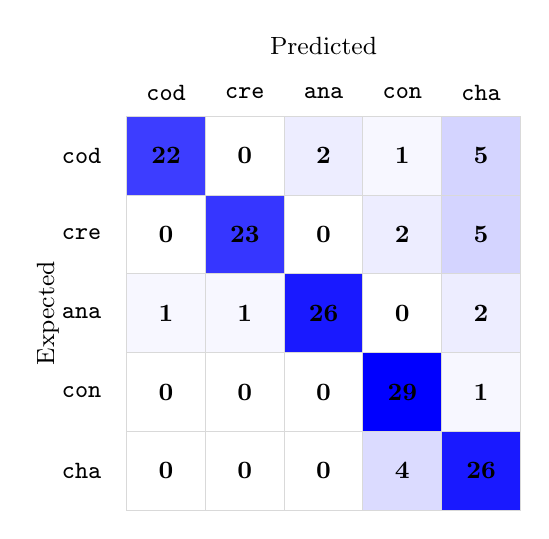
\begin{tikzpicture}[cell/.style={minimum size=1cm, draw=gray!30, font=\small\bfseries}]
  % Row 0: code (expected) -- 22 0 2 1 5
  \node[cell, fill=blue!76] at (0, 0) {22};
  \node[cell, fill=blue!0]  at (1, 0) {0};
  \node[cell, fill=blue!7]  at (2, 0) {2};
  \node[cell, fill=blue!3]  at (3, 0) {1};
  \node[cell, fill=blue!17] at (4, 0) {5};
  % Row 1: creative -- 0 23 0 2 5
  \node[cell, fill=blue!0]  at (0,-1) {0};
  \node[cell, fill=blue!79] at (1,-1) {23};
  \node[cell, fill=blue!0]  at (2,-1) {0};
  \node[cell, fill=blue!7]  at (3,-1) {2};
  \node[cell, fill=blue!17] at (4,-1) {5};
  % Row 2: analytical -- 1 1 26 0 2
  \node[cell, fill=blue!3]  at (0,-2) {1};
  \node[cell, fill=blue!3]  at (1,-2) {1};
  \node[cell, fill=blue!90] at (2,-2) {26};
  \node[cell, fill=blue!0]  at (3,-2) {0};
  \node[cell, fill=blue!7]  at (4,-2) {2};
  % Row 3: conversational -- 0 0 0 29 1
  \node[cell, fill=blue!0]   at (0,-3) {0};
  \node[cell, fill=blue!0]   at (1,-3) {0};
  \node[cell, fill=blue!0]   at (2,-3) {0};
  \node[cell, fill=blue!100] at (3,-3) {29};
  \node[cell, fill=blue!3]   at (4,-3) {1};
  % Row 4: chaotic -- 0 0 0 4 26
  \node[cell, fill=blue!0]  at (0,-4) {0};
  \node[cell, fill=blue!0]  at (1,-4) {0};
  \node[cell, fill=blue!0]  at (2,-4) {0};
  \node[cell, fill=blue!14] at (3,-4) {4};
  \node[cell, fill=blue!90] at (4,-4) {26};
  % Column labels (predicted)
  \foreach \lbl [count=\x from 0] in {cod,cre,ana,con,cha} {
    \node[font=\small] at (\x, 0.8) {\texttt{\lbl}};
  }
  % Row labels (expected)
  \foreach \lbl [count=\y from 0] in {cod,cre,ana,con,cha} {
    \node[font=\small, anchor=east] at (-0.7, -\y) {\texttt{\lbl}};
  }
  \node[font=\small] at (2, 1.4) {Predicted};
  \node[font=\small, rotate=90] at (-1.5, -2) {Expected};
\end{tikzpicture}
\caption{Confusion matrix for AutoTune context classification ($n=150$). The \texttt{chaotic} class acts as an attractor, absorbing 13 false positives from other classes.}
\label{fig:confusion}
\end{figure}

\paragraph{Baseline comparison.} We compare against four baselines (Table~\ref{tab:baselines}): random (uniform), majority class, message-length heuristic, and flat keyword counting (same patterns, no $3\times$ message weighting).

\begin{table}[t]
\caption{Baseline comparison with 95\% bootstrap confidence intervals ($B=10{,}000$).}
\label{tab:baselines}
\centering
\small
\begin{tabular}{@{}lccc@{}}
\toprule
Classifier & Accuracy & 95\% CI & Macro F1 \\
\midrule
\textbf{AutoTune (proposed)} & \textbf{84.0\%} & \textbf{[78.0, 89.3]} & \textbf{84.2\%} \\
Keyword count (flat) & 78.7\% & [72.0, 84.7] & 80.0\% \\
Length heuristic & 25.3\% & [18.7, 32.7] & 21.1\% \\
Random (uniform) & 20.4\% & [19.8, 21.1] & 20.4\% \\
Majority class & 20.0\% & [14.0, 26.7] & 6.7\% \\
\bottomrule
\end{tabular}
\end{table}

\begin{figure}[t]
\centering
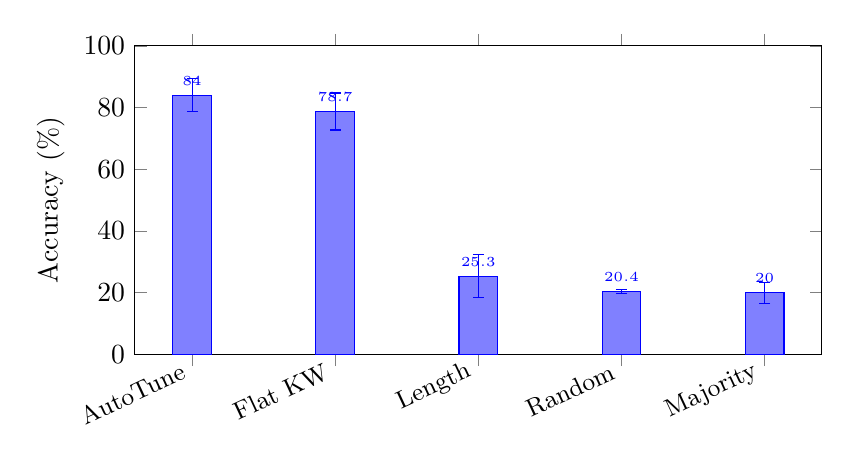
\begin{tikzpicture}
\begin{axis}[
    ybar,
    bar width=14pt,
    ylabel={Accuracy (\%)},
    symbolic x coords={AutoTune,Flat KW,Length,Random,Majority},
    xtick=data,
    xticklabel style={rotate=25, anchor=east, font=\small},
    ymin=0, ymax=100,
    nodes near coords,
    nodes near coords style={font=\tiny},
    width=0.85\linewidth,
    height=5.5cm,
    every node near coord/.append style={above},
]
\addplot+[
    fill=blue!50,
    error bars/.cd, y dir=both, y explicit,
] coordinates {
    (AutoTune, 84.0) +- (0, 5.3)
    (Flat KW, 78.7) +- (0, 6.0)
    (Length, 25.3) +- (0, 7.0)
    (Random, 20.4) +- (0, 0.6)
    (Majority, 20.0) +- (0, 3.4)
};
\end{axis}
\end{tikzpicture}
\caption{Baseline comparison with 95\% bootstrap CIs. AutoTune improves +5.3\,pp over the strongest baseline (McNemar $\chi^2 = 3.06$, $p \approx 0.08$).}
\label{fig:baselines}
\end{figure}

AutoTune improves +5.3\,pp absolute over the strongest baseline (flat keyword counting). McNemar's test yields $\chi^2 = 3.06$, $p \approx 0.08$---suggestive but not significant at $\alpha = 0.05$ with $n=150$. The effect size is modest: Cohen's $h = 0.14$ for the accuracy difference, placing this in the ``small effect'' range~\cite{cohen1988statistical}. Per-class analysis shows the $3\times$ message weighting helps conversational (+20.5 F1\,pp) but hurts chaotic ($-$13.9 F1\,pp) by amplifying the attractor effect.

\paragraph{Statistical power.} With $n=150$ (30 per class), a post-hoc power analysis indicates approximately 42\% power to detect a 5.3\,pp improvement at $\alpha=0.05$. Achieving 80\% power would require $n \approx 400$. We therefore characterize the AutoTune advantage over flat keyword counting as \emph{suggestive} rather than \emph{conclusive}, and note that the primary value of context-adaptive parameter selection lies in its transparency and traceability rather than in marginal accuracy gains.

\paragraph{Accuracy by difficulty.} Easy: 96.0\% (72/75), Medium: 88.0\% (44/50), Hard: 40.0\% (10/25). Hard cases expose the regex approach's inability to classify keyword-free messages.

\paragraph{Confidence anti-calibration.} Average confidence for correct predictions (65.2\%) is \emph{lower} than for incorrect predictions (76.4\%), a separation of $-11.2$\,pp. The chaotic category's aggressive patterns produce high-confidence scores even on misclassified inputs.

\subsection{Feedback Loop Convergence}

\paragraph{Setup.} We simulate 5 synthetic users with defined preferred/disliked parameter vectors. Each generates alternating $+1$/$-1$ ratings over 50 steps. We measure normalized L2 distance to the user's preferred parameters.

\begin{table}[t]
\caption{Feedback convergence results (50 ratings, 0\% noise).}
\label{tab:convergence}
\centering
\small
\begin{tabular}{@{}llcccc@{}}
\toprule
Profile & Context & Init.\ Dist. & Final Dist. & Improv. & Cold Start \\
\midrule
CodePrecisionist & code & 0.186 & 0.108 & 42.1\% & Step 3 \\
CreativeWriter & creative & 0.222 & 0.138 & 37.9\% & Step 3 \\
DataAnalyst & analytical & 0.105 & 0.041 & 61.5\% & Step 3 \\
CasualChatter & convers. & 0.042 & 0.026 & 38.2\% & Step 3 \\
ChaosAgent & chaotic & 0.327 & 0.232 & 29.2\% & Step 3 \\
\bottomrule
\end{tabular}
\end{table}

\begin{figure}[t]
\centering
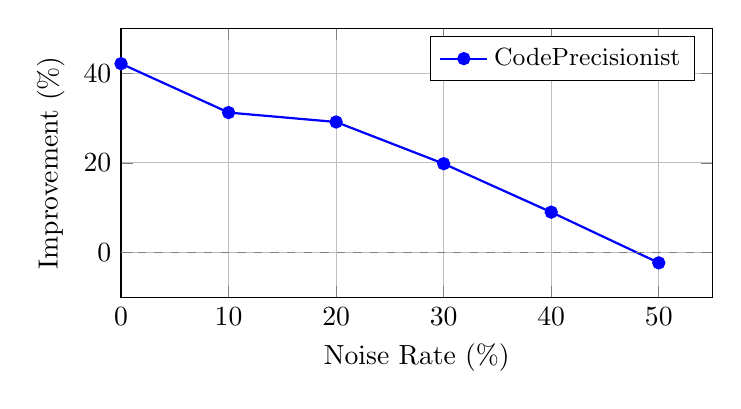
\begin{tikzpicture}
\begin{axis}[
    xlabel={Noise Rate (\%)},
    ylabel={Improvement (\%)},
    xmin=0, xmax=55,
    ymin=-10, ymax=50,
    grid=major,
    width=0.75\linewidth,
    height=5cm,
    mark size=2pt,
    legend pos=north east,
    legend style={font=\small},
]
\addplot[blue, thick, mark=*] coordinates {
    (0, 42.1) (10, 31.2) (20, 29.1) (30, 19.8) (40, 9.0) (50, -2.3)
};
\addlegendentry{CodePrecisionist}
\addplot[dashed, gray] coordinates {(0,0) (55,0)};
\end{axis}
\end{tikzpicture}
\caption{Noise robustness of the feedback loop (CodePrecisionist profile, 50 ratings, averaged over 5 runs). The system degrades gracefully and correctly produces ${\approx}0$ adjustment at 50\% noise.}
\label{fig:noise}
\end{figure}

\paragraph{Convergence speed.} For 4/5 profiles, 50\% of maximum improvement is reached at step 12, 75\% at step 16, and 90\% at step 19.

\paragraph{Noise robustness.} At 20\% noise (1 in 5 ratings flipped), the system still achieves 29.1\% improvement. At 50\% (random), it correctly produces near-zero net adjustment ($-$2.3\%), confirming uniform noise cancels as expected (Figure~\ref{fig:noise}).

\subsection{STM Precision and Recall}

We construct 77 test cases: 26 for \texttt{hedge\_reducer} (16+, 10$-$), 21 for \texttt{direct\_mode} (11+, 10$-$), 30 for \texttt{casual\_mode} (20+, 10$-$). All three modules achieve \textbf{100\% precision, 100\% recall, 100\% F1} on the test set. Pipeline composition achieves 29.5--48.6\% character reduction. We note this reflects deterministic regex matching on constructed cases; coverage against real-world outputs is untested.

\subsection{ULTRAPLINIAN Scoring Calibration}

\begin{table}[t]
\caption{Quality tier discrimination of the scoring function.}
\label{tab:tiers}
\centering
\small
\begin{tabular}{@{}llc@{}}
\toprule
Tier & Configuration & Score \\
\midrule
Excellent & 2000 chars, 4 headers, 8 list, 2 code, direct, relevant & 98 \\
Good & 800 chars, 2 headers, 3 list, 1 code, direct, relevant & 89 \\
Mediocre & 300 chars, 1 header, preamble, relevant & 57 \\
Poor & 200 chars, no structure, preamble, 1 refusal, relevant & 43 \\
Terrible & 150 chars, no structure, preamble, 3 refusals, irrelevant & 16 \\
\bottomrule
\end{tabular}
\end{table}

\begin{figure}[t]
\centering
\begin{tikzpicture}
\begin{axis}[
    xbar,
    bar width=10pt,
    xlabel={Score Change ($\Delta$)},
    symbolic y coords={Relevance,Preamble,Structure,Refusals,Length},
    ytick=data,
    xmin=-50, xmax=0,
    width=0.8\linewidth,
    height=5cm,
    nodes near coords,
    nodes near coords style={font=\small, anchor=east},
    every node near coord/.append style={xshift=-3pt},
]
\addplot[fill=red!50] coordinates {
    (-43, Length)
    (-24, Refusals)
    (-19, Structure)
    (-10, Relevance)
    (-7, Preamble)
};
\end{axis}
\end{tikzpicture}
\caption{Scoring component contribution analysis. Degrading each component individually from a baseline score of 92. Length dominates at 46.7\% of the score range.}
\label{fig:components}
\end{figure}

All five quality tiers are strictly ordered ($98 > 89 > 57 > 43 > 16$; spread: 82 points). Length monotonicity is confirmed. Component analysis (Figure~\ref{fig:components}) reveals length contributes 46.7\% of the effective score range, followed by anti-refusal (26.1\%), structure (20.7\%), relevance (10.9\%), and directness (7.6\%).

\subsection{Parseltongue Transformation Analysis}

All 54 triggers (53 unique) achieve 100\% detection across 6 positional variations. Table~\ref{tab:parseltongue} shows per-technique properties at medium intensity. Leetspeak produces the highest edit distance (8.6); unicode is length-preserving; phonetic is deterministic (1 variant). Intensity scaling is monotonic across all techniques.

\begin{table}[t]
\caption{Parseltongue per-technique properties (medium intensity, 5 runs).}
\label{tab:parseltongue}
\centering
\small
\begin{tabular}{@{}lccccc@{}}
\toprule
Technique & Edit Dist. & Non-ASCII & Zero-Width & $\Delta$Len & Variants \\
\midrule
\textsc{leetspeak} & 8.6 & 2.4 & 0 & +2.6 & 10/10 \\
\textsc{unicode}   & 6.0 & 6.0 & 0 & 0    & 10/10 \\
\textsc{zwj}       & 6.0 & 6.0 & 6.0 & +6.0 & 10/10 \\
\textsc{mixedcase} & 5.0 & 0   & 0 & 0    & 10/10 \\
\textsc{phonetic}  & 3.0 & 0   & 0 & 0    & 1/10 \\
\textsc{random}    & 6.6 & 1.8 & 0 & +1.0 & 10/10 \\
\bottomrule
\end{tabular}
\end{table}

%==============================================================================
% 6. DISCUSSION
%==============================================================================
\section{Discussion}

\paragraph{Output steering as a unified phenomenon.}
The central finding is not that any individual module is novel in isolation---regex classifiers, EMA estimators, and character substitutions are well-understood techniques. The contribution is framing these as \emph{composable steering primitives} over a shared control surface. The same AutoTune parameter that suppresses creative outputs in code contexts ($\tau=0.15$) amplifies them in creative contexts ($\tau=1.15$). The same ULTRAPLINIAN scoring that selects for safety compliance (high $S_{\text{anti}}$) can, with reweighted axes, select for pedagogical structure or technical depth. This composability suggests that inference-time output steering is a richer design space than either the safety community (which focuses on attack/defense) or the controllable generation community (which focuses on model internals) has fully mapped.

\paragraph{Implications for alignment.}
The malleability of LLM outputs to inference-time intervention has direct implications for alignment research. If sampling parameters, input perturbations, and multi-model selection can substantially shift output distributions \emph{without touching weights}, then safety training must be robust not only to adversarial prompts but to the full compositional space of API-level interventions. Our results quantify pieces of this: AutoTune's 5 context profiles span a parameter range from $\tau=0.15$ to $\tau=1.70$; Parseltongue's 6 techniques produce edit distances up to 8.6 characters per trigger; ULTRAPLINIAN's 27-model races expose systematic cross-provider variation. Each primitive alone is modest; composed, they multiply.

\paragraph{Transparency as a design choice.}
AutoTune's 20 regex patterns achieve 84.0\% accuracy---well above trivial baselines but only +5.3\,pp over flat keyword counting (not significant at $\alpha=0.05$; Cohen's $h=0.14$, small effect). We could improve accuracy with learned classifiers, but transparency is a deliberate choice: every context classification can be traced to specific pattern matches, enabling researchers (and users) to understand exactly why the system steered in a particular direction. The chaotic attractor amplification ($-$13.9 F1\,pp) is the primary failure mode and a direct consequence of this transparency tradeoff. We stress that these computational evaluations measure the steering primitives themselves---they do not constitute evidence that steered outputs are \emph{effective} at any downstream task, nor that Parseltongue perturbations succeed against any specific model's safety training in practice.

\paragraph{Scoring policy determines behavior.}
ULTRAPLINIAN's length axis contributes 46.7\% of the effective score range (Figure~\ref{fig:components}). This is not a flaw but a policy choice: the default scoring favors comprehensive responses. Reweighting toward anti-refusal and directness produces a very different selection policy. The interpretable, axis-based scoring enables researchers to define precisely what ``best response'' means for their steering objective, making the value alignment of the scoring function itself legible and auditable.

\paragraph{Limitations.}
\begin{enumerate}
    \item The chaotic attractor (66.7\% precision) may steer outputs under incorrect parameter configurations.
    \item Confidence scores are anti-calibrated ($-$11.2\,pp)---should not gate steering decisions.
    \item STM 100\% accuracy reflects deterministic matching on constructed cases, not real-world coverage.
    \item The feedback loop's 50\% cap limits maximum adaptation to 29--62\%.
    \item Single-provider dependency (OpenRouter) limits reproducibility.
    \item Phonetic technique is fully deterministic (1 variant)---provides no perturbation diversity.
    \item Interaction effects between composed primitives are not yet evaluated.
    \item No claims about effectiveness against any specific model's safety training. We emphasize that computational evaluation of steering primitives does not constitute evidence of real-world impact on model behavior in deployed settings; real-user studies are needed to establish practical effectiveness.
\end{enumerate}

\paragraph{Threats to validity.}
\emph{Internal validity:} All test sets (150 classification instances, 77 STM cases, 5 synthetic feedback profiles) were constructed by the authors. No external annotators were used; inter-annotator agreement is therefore unreported. The self-constructed nature of these benchmarks may introduce systematic biases toward patterns the system was designed to handle.
\emph{External validity:} All evaluations are computational---no real-user studies, A/B tests, or in-the-wild deployments are reported. The synthetic feedback profiles simulate idealized user behavior (consistent preferences, uniform rating schedules) that may not reflect real usage patterns. Results may not generalize to production environments with diverse user populations.
\emph{Construct validity:} The ULTRAPLINIAN scoring function and AutoTune context categories reflect design choices, not ground-truth constructs. The five scoring axes and their relative weights encode assumptions about what constitutes response quality; alternative axis designs could yield different selection behavior.
\emph{Statistical power:} With $n=150$ for AutoTune classification, the study is underpowered to detect small effects. McNemar's test yields $p=0.08$, which does not reach significance at $\alpha=0.05$. A post-hoc power analysis indicates that detecting a 5.3\,pp improvement with 80\% power at $\alpha=0.05$ would require approximately $n \approx 400$ samples. We report the improvement as suggestive, not conclusive.

\paragraph{Ethical considerations.}
The three-tier data collection architecture (\S\ref{sec:datacollection}) was designed with a privacy-by-construction approach: Tiers~1 and~2 structurally exclude message content, prompts, responses, and PII at the code level, not via post-hoc filtering. Tier~3 (full steering context including messages and responses) requires explicit opt-in from the caller. All collected data is published as open datasets on HuggingFace.
Parseltongue's character-level perturbation techniques probe the robustness of model safety training, raising dual-use concerns addressed in the Broader Impact Statement. We note that these techniques are individually well-known; the framework's contribution is systematization, not novelty of attack surface.
We recommend that vulnerability findings obtained using this framework be reported to model providers via responsible disclosure before public dissemination. This project has not undergone formal IRB or ethics board review, as it does not involve human subjects research in the traditional sense; however, we acknowledge that deployed steering tools interact with real users and recommend that future work involving human evaluation of steered outputs seek appropriate oversight.

%==============================================================================
% DEPLOYMENT AND RESPONSIBLE USE
%==============================================================================
\section{Deployment Considerations}
\label{sec:deployment}

G0DM0D3 is deployed as a public research preview at a dedicated domain, making responsible deployment an active concern rather than a theoretical one. We describe the measures taken and the rationale behind them.

\paragraph{Terms of service and informed consent.} A mandatory first-visit disclaimer requires users to acknowledge that (1) they are solely responsible for generated outputs, (2) the tool is provided as-is for research purposes, (3) they will not generate content violating applicable laws, and (4) the developers assume no liability for third-party model outputs. Users must explicitly accept before accessing the interface.

\paragraph{Client-side architecture.} All API keys are stored exclusively in the user's browser localStorage and never transit our infrastructure. No conversations are logged, stored, or monitored server-side. This privacy-first architecture means we cannot perform content moderation on user queries, which we view as an acceptable tradeoff for a research tool: the models themselves retain their safety training, and the responsibility boundary is clearly communicated.

\paragraph{Three-tier data collection.} Users should be aware that the deployment collects metadata at three levels (\S\ref{sec:datacollection}, Table~\ref{tab:datacollection}). Tiers~1 (ZDR server-side metadata) and~2 (client-side telemetry beacon) are always active and record only structural metadata---endpoints, models, latencies, pipeline flags, and scores---never message content, prompts, responses, API keys, or PII. Tier~3 (dataset collection) is strictly opt-in: it activates only when the caller explicitly passes \texttt{contribute\_to\_dataset: true}, and records the full steering context including messages and responses but still excludes API keys and IP addresses. All tiers auto-publish to HuggingFace as open datasets. This design ensures that passive data collection cannot reconstruct any user's conversation, while opt-in collection provides rich steering data for the research community.

\paragraph{Security hardening.} Content Security Policy headers restrict script execution and connection targets. Backend source code, configuration files, and API documentation are blocked from public access via static hosting rules. Cross-origin policies prevent embedding and resource theft. Rate limiting (configurable per deployment) bounds API throughput.

\paragraph{Open-source transparency.} The full codebase---including all system prompts, perturbation techniques, scoring functions, and data collection implementations---is publicly available. We believe this transparency serves safety better than obscurity: published steering techniques enable model providers to test and strengthen defenses, the data collection code is fully auditable, and the research community can study inference-time malleability systematically rather than rediscovering it ad-hoc.

%==============================================================================
% BROADER IMPACT
%==============================================================================
\section*{Broader Impact Statement}

\paragraph{The case for open steering research.} G0DM0D3 makes explicit a control surface that already exists in every LLM API. Sampling parameters, system prompts, and model selection are available to every API user; Parseltongue's character-level perturbations are techniques discovered independently by countless users. By systematizing these into a research framework with measurable, reproducible primitives, we aim to advance understanding of inference-time malleability---both its productive applications (better creative tools, adaptive tutoring, personalized assistants) and its risks (safety bypass, output manipulation).

\paragraph{Dual-use reality.} The same framework that enables a researcher to evaluate safety training robustness enables a user to steer toward unrestricted outputs. We address this honestly: (1) the techniques are well-documented character-level transformations and sampling configurations, not novel attack vectors unavailable elsewhere; (2) open-source publication enables defensive research and countermeasure development by model providers; (3) the configurable scoring axes make the steering objective legible and auditable; (4) mandatory terms of service place responsibility on the user.

\paragraph{What this framework reveals.} The deeper implication is that LLM outputs are more malleable to inference-time intervention than safety training alone can address. This is not an argument against safety training---it is an argument that safety must be evaluated against the full compositional space of API-level interventions, and that the research community needs open tools to map this space systematically.

\paragraph{Recommendations.} (1) Downstream content filtering for production deployments using this framework; (2) Parseltongue perturbation studies in controlled settings with appropriate oversight; (3) vulnerability findings reported to model providers via responsible disclosure; (4) continued development of safety training robust to the compositional steering surface this work characterizes.

%==============================================================================
% CONCLUSION
%==============================================================================
\section{Conclusion}

We have presented \textsc{G0DM0D3}, a framework for inference-time LLM output steering comprising five composable, objective-agnostic primitives. AutoTune achieves 84.0\% context classification accuracy [78.0, 89.3] over four baselines, enabling automatic sampling adaptation. The EMA-based feedback loop converges to 29--62\% parameter improvement within 19 ratings. Parseltongue systematizes character-level input perturbation across six techniques and three intensity levels. STM provides composable output normalization. ULTRAPLINIAN achieves strict quality-tier ordering with 82-point discrimination across up to 27 models.

The framework's central contribution is conceptual: these primitives compose. Sampling control, input perturbation, multi-model selection, preference learning, and output shaping operate on different control surfaces but toward a shared steering objective determined entirely by configuration. This composability reveals inference-time output steering as a richer design space than previously characterized---one that alignment research, controllable generation, and practical LLM application development all need to engage with.

The system is deployed as a public research preview with mandatory terms of service, client-side-only credential storage, and full open-source transparency. All code and evaluation scripts are available (repository link withheld for review).

\paragraph{Future directions.} (1) Interaction effects: evaluating how composed primitives amplify or interfere with each other across the full combinatorial space. (2) Learned steering: replacing regex-based context detection with lightweight classifiers while preserving transparency. (3) Objective-specific scoring profiles: curated ULTRAPLINIAN weight sets for safety evaluation, creative writing, technical instruction, and other domains. (4) Cross-provider steering maps: using ULTRAPLINIAN races to characterize how different models respond to the same steering interventions, building an empirical atlas of inference-time malleability.

%==============================================================================
% REFERENCES
%==============================================================================
\bibliographystyle{plainnat}
\bibliography{references}

%==============================================================================
% APPENDIX
%==============================================================================
\newpage
\appendix
\section{Reproducibility Checklist}

\begin{table}[h]
\centering
\small
\begin{tabular}{@{}lp{8cm}@{}}
\toprule
Item & Status \\
\midrule
Source code & Yes --- repository withheld for review \\
Hyperparameters & Yes --- Tables~\ref{tab:profiles}, EMA $\alpha=0.3$, scoring weights in \S\ref{sec:ultraplinian} \\
Regex patterns & Yes --- inspectable in source \\
Scoring function & Yes --- 5 components with exact formulas \\
Evaluation scripts & Yes --- \texttt{research/eval\_*.ts} \\
Statistical tests & Yes --- Bootstrap CIs, McNemar's test \\
Training data & \textbf{None} --- system is training-free \\
Compute & Minimal --- TypeScript, no GPU \\
Deployment config & Yes --- security headers, ToS, privacy architecture documented \\
Metadata schema & Yes --- three-tier collection (ZDR, telemetry, opt-in dataset) with field-level documentation in \S\ref{sec:datacollection} and Table~\ref{tab:datacollection} \\
\bottomrule
\end{tabular}
\end{table}

\end{document}
